\chapter{Material and Methods}
\label{chap:material}
Simulating ultrasound data can be an extremely useful technique to thoroughly test different setups. Unlike real data recording, simulations allow full control of the setups parameters.
One of the most widely used programs for ultrasound imaging simulations is the \textit{Field II Simulation Program}  created by Professor Jørgen Arendt Jensen at the Technical University of Denmark (\cite{Field_II, Field_II_ext}). All simulations produced in this thesis are done in MATLAB using Field II.

\section{Simulation parameters}
\label{sec:sim_param}
In all the simulations, the simulated ultrasound probe consists of a linear array of 96 transducers all transmitting at $f_c = 3~$MHz center frequency with a bandwidth of $2.3~$MHz (77\%). They are also all serving the dual function of recording ultrasound data at the same center frequency and bandwidth. The recorded data is sampled at $90~$MHz sampling frequency. Each transducer has a height of $10~$mm and a width of $0.24~$mm. The transducer's \textit{pitch}, defined as the distance from a transducer's center to the center of its neighboring one, is set to $d = \lambda / 2~$m, where $\lambda$ is the wavelength of the transducer's center frequency.
The speed of ultrasound propagation $c$ in a medium can vary significantly depending, among other parameters, on the imaged medium temperature and content, whether it is fatty or non-fatty tissue, bone, liver, any other organ or a combination of those. \cite{Ultrasound_propagation} showed that $c$ is most often lies in the $1400-1600~$m/s range. In this thesis, $c$ is set to $1500~$m/s.

The transducer's pitch is then $d = \lambda / 2 = c / (2 \cdot f_c) = 1500 / (2\cdot3\cdot10^6) = 0.25~$mm. With a \textit{kerf}, or distance between transducers, of $0.01~$mm, the transducer's width is then of $0.24~$mm (pitch minus kerf) and the total length of the array is $96 \cdot 0.25 = 24~$mm.

A signal pulse $s(t)$ is created by simulating an excitation in the form of alternative voltage of period $T = 2\pi$:
\begin{equation}
    s(t) = \left \{ \begin{tabular}{cc}
        1, & $0 \leq t < \pi$ \\
        -1, & $\pi \leq t < 2\pi$
    \end{tabular}\right..
\end{equation}
\noindent
The transducer's output pulse is defined by the excitation function convolved with the transducer's impulse response $h_t(t)$.
In this thesis, $h_t(t)$ is implemented as a bandpass filter around the pulse's center frequency ($3~$MHz) using a Blackman window (\cite{blackman}). The same impulse response is used for signals reception ($h_r(t) = h_t(t)$). The medium and backscatterer points are assumed to be ideal in the sense that they do not alter the signals properties. This means that $s(t) * h_m(t) * h_p(t) * h_m(t) = s(t)$, where $h_m(t)$ is the medium's impulse response and $h_p(t)$ the one of the scatterer point. The medium's impulse response is applied twice since the signal is traveling from the array to the scatterer point and back.
Under those conditions, a signal pulse $s(t)$ sent by a transducer, backscattered by a point in the medium, and recorded by a transducer can be defined as:
\begin{align}
    y(t) &= s(t) * h_t(t) * h_m(t) * h_p(t) * h_m(t) * h_r(t) \nonumber \\
    &= s(t) * h_t(t) * h_t(t),
\end{align}
\noindent
where $*$ is the convolution operator. The perceived pulse $y(t)$ is illustrated in Figure \ref{fig:pulse}.

\begin{figure}
    \centering
    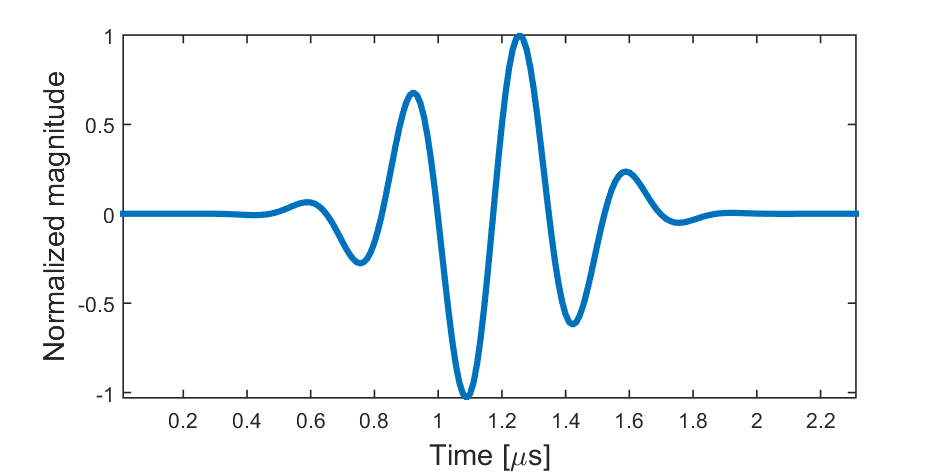
\includegraphics[width=\linewidth]{./images/others/pulse.png}
    \caption{Simulated signal pulse on reception}
    \label{fig:pulse}
\end{figure}

The imaged section is chosen to span from $-17.5$ to $17.5^\circ$ from the array's normal vector, and $35$ to $60~$mm range to it. The aperture default focus is set to $40~$mm radius. Note that this thesis differentiates the terms \textit{radius}, which defines the absolute distance to the array center in any direction, and \textit{range}, which defines the radius projection onto the array's normal plane. A point's \textit{azimuth} is its radius projection onto the array's parallel plane.

All transmit or receive beams are focused at the same radius ($40~$mm) and distributed uniformly along the imaged azimuth sector. In other words, the beams distribution is uniform in $sin(\theta_b)$, where $\theta_b$ is the direction angle of beam $b$ from the array center.
The beams with outermost direction $\theta_b$ from the array center are set to $sin(\theta_b)$ = -0.3 and 0.3.
For any given range $r$, the azimuth distance $d_B$ between two transmit beams is a constant value:
\begin{align}
    d_B = 0.3 \cdot r / \lfloor b_{tr} / 2 \rfloor,
\label{eq:dist_beams}
\end{align}
\noindent
where $b_{tr}$ is the number of beams used to illuminate the imaged sector and $\lfloor \rfloor$ is the floor operator.

Unless specified otherwise, all beamformed images are built by sequentially transmitting beams in various directions and, for each transmit beam, focusing the array towards that same direction during receive. The number of receive beams $b_{re}$ is then equal to the number of transmit beams $b_{tr}$. This approach is often referred to as single-line acquisition (SLA).
In practice, a lot of beamformers are configured to use parallel-receive beamfoming (PRB), also known as multiple-line acqusition (MLA), presented in Section \ref{sec:prb}. The purpose of PRB is to improve a beamformer's frame rate by reducing the number of transmit beams while maintaining a similar resolution level by increasing the number of receive beams.
However, this approach has shown to induce artifacts and various PRB approaches have been introduced to try to limit those artifacts (\cite{multiline}).
In order to avoid this problematic, perfect PRB is simulated in this thesis by upsampling the number of transmit beams and using SLA. Assuming perfect PRB, an image built from $b_{tr} = b_{re} = 195$ beams can therefore also be seen as built from $b_{tr} = 65$ transmit beams and $b_{re} = 3 \cdot b_{tr} = 195$ receive beams, or $b_{tr} = 39$ and $b_{re} = 5 \cdot b_{tr} = 195$ beams.

The imaged medium contains scatterer points either in a noiseless medium or in a \textit{speckle} background, depending on the experiment. Speckle noise consists of the transmitted signals scattered by a large number of small, densely distributed, scatterer points and is used to simulate homogeneous tissues.
The noiseless background scenario is a very controlled setup, with no randomness in the medium which could possibly alter the results. It is typically run first and its results are used to make fundamental observations and in-depth analysis. The speckle scenario is a more realistic one, typically used to verify the observations from the first scenario and obtain qualitative results closer to those of a real use case.
This thesis focuses on noiseless media, but provides an exposure to more realistic media with two examples of randomly-generated speckle background.
Due to the randomness of the speckle noise, a thorough analysis of the influence of motion with the presence of speckle noise would require to run the same experiments with dozens or even hundreds of different randomly-generated speckle backgrounds to be statistically meaningful.
The speckle simulations are therefore targeted to be used as examples of realistic divergences from the noiseless medium and not data of statistical significance.
In this thesis, speckle is generated by simulating one million small scatterer points uniformly distributed along the full image plane, covering -90 to 90 degrees angular span and 5 to 75 mm range.
Figure \ref{fig:speckle} displays DAS beamformed images of the two speckle backgrounds used in this thesis.

The parameters used for the aperture and medium simulation are summarized in Tables \ref{table:aperture_param} and \ref{table:medium_param}.

\begin{figure}[ht]
    \centering
    \begin{subfigure}[t]{0.48\linewidth}
        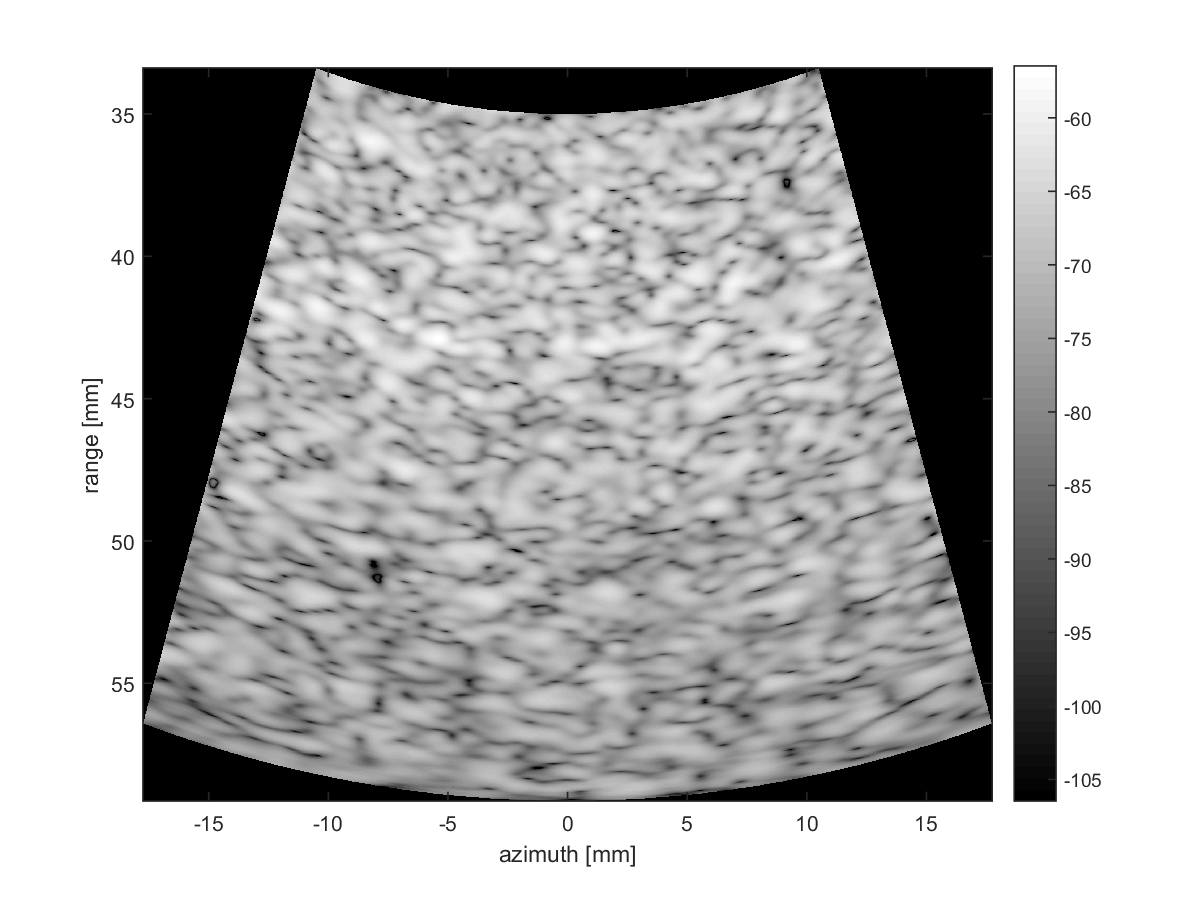
\includegraphics[width=\linewidth]{./images/results/2.3/speckle2.png}
        \caption{Speckle seed = 2}
    \end{subfigure}
    \quad
    \begin{subfigure}[t]{0.48\linewidth}
        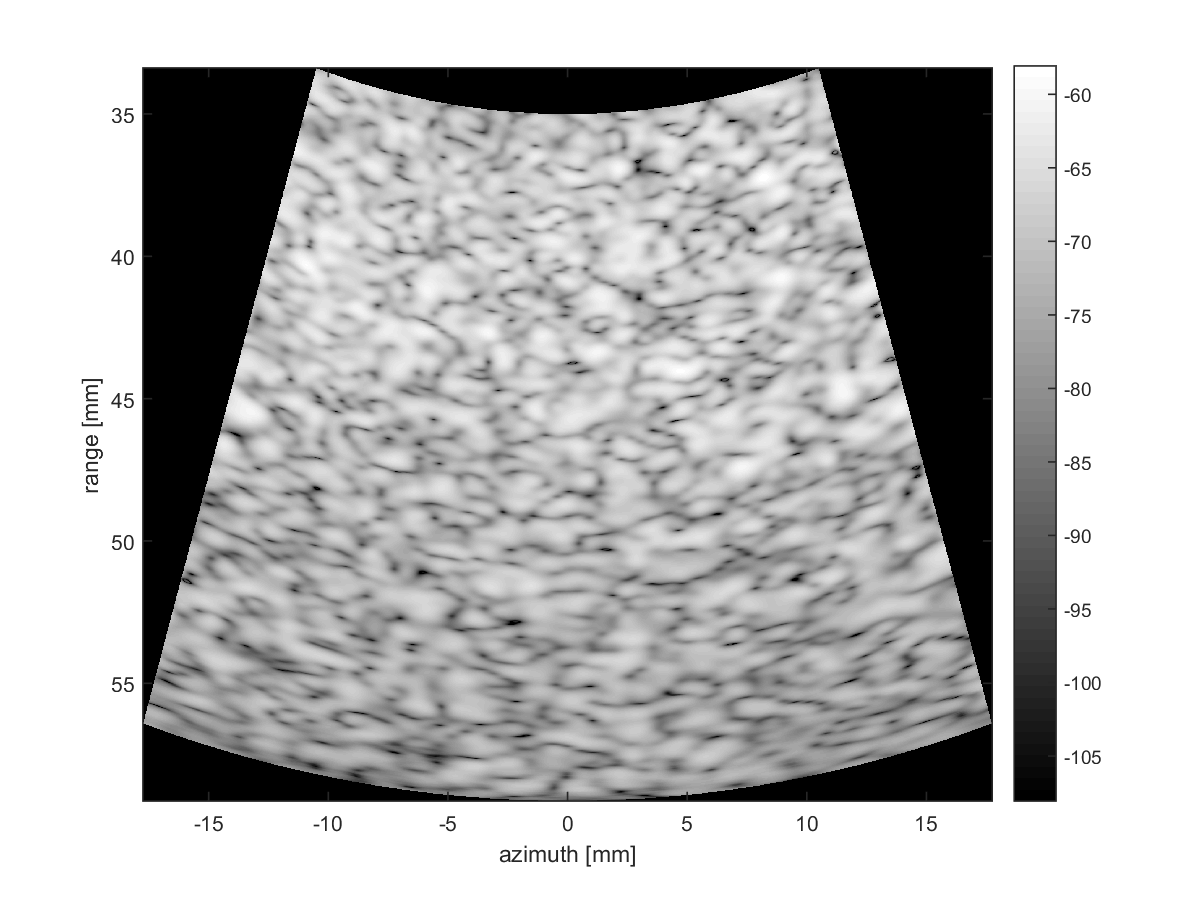
\includegraphics[width=\linewidth]{./images/results/2.3/speckle42.png}
        \caption{Speckle seed = 42}
    \end{subfigure}
	\caption{DAS beamformer image of speckle background with $b_{tr}=65$ transmit beams}
	\label{fig:speckle}
\end{figure}

\iffalse
  Recorded frequencies bandwidth    &   1.8457 - 4.1528 MHz
  along the full image plane, covering the full -90 to 90 degrees angular span.
\fi


\begin{table}[!ht]
\centering
\begin{tabular}{|*{2}{c|}}
 \hline
 \multicolumn{2}{c}{Probe parameters} \\
  \hline
  Transmit and record center frequency    &   3 MHz \\
  Transmit and record frequency bandwidth    &   2.3 MHz \\
  Sampling frequency    &   90 MHz \\
  Number of transducers &   96 \\
  Transducer height   &   10 mm \\
  Transducer width   &   0.24 mm \\
  Transducer pitch   &   0.25 mm \\
  Kerf   &   0.01 mm \\
  Array length   &   24 mm \\
  \hline
  \multicolumn{2}{c}{} \\
  
  \hline
  \multicolumn{2}{c}{Default aperture parameters} \\
  \hline
  Imaging sector  &   -17.5 to 17.5 degrees \\
  Imaging range     &   35 to 60 mm \\
  Radial focus   &   40 mm \\
  Impulse response window   &   Blackman \\
  Distribution of transmit beams   &   Uniform along azimuth \\
  Distribution of receive beams   &   Matching transmit \\
  \hline
 \end{tabular}
\caption{Probe parameters}
\label{table:aperture_param}
\end{table}
  
\begin{table}[!ht]
\centering
\begin{tabular}{|*{2}{c|}}
 \hline
 \multicolumn{2}{c}{Medium parameters} \\
  \hline
  Speed of propagation    &   1500 m/s \\
  Speckle sector    &   -90 to 90 degrees \\
  Speckle range     &   5 to 75 mm \\
  Speckle azimuth   &   -75 to 75 mm \\
  Speckle distribution  &   Uniformly distributed \\
  Number of points in speckle    &   $10^6$ \\
  Random generator seed     &   2 and 42 \\
  Scatterer points amplitude   &   30 dB over speckle \\
  \hline
 \end{tabular}
\caption{Medium parameters}
\label{table:medium_param}
\end{table} 

\section{Beamformers parameters}
\label{sec:beamform_param}
Four different beamforming algorithms are implemented and tested in this thesis:
\begin{itemize}
    \item DAS: Conventional Delay-And-Sum beamforming (Section \ref{sec:DAS})
    \item MV: Minimum-Variance beamforming (Section \ref{sec:MV})
    \item IAA-MB: Iterative Adaptive Approach (Section \ref{sec:IAA}). Two variants of the algorithm are compared:
    \subitem IAA-MBSB: (Multibeam/Singlebeam) The MB approach is used during the iteration stage and the SB approach for the final sources amplitude.
    \subitem IAA-MBMB: (Multibeam/Multibeam) The MB approach is used both during the iteration stage and the final sources amplitude estimation.
\end{itemize}
\noindent
As explained in section \ref{sec:MV}, the MV beamformer in its standard form is prone to artifacts and requires some robustification improvements. In this thesis, the MV beamformer is enhanced with the use of spatial smoothing, diagonal loading, temporal averaging and forward-backward averaging (Sections \ref{sec:diagonal_loading}, \ref{sec:spatial_smoothing}, \ref{sec:time_averaging} and \ref{sec:fb_averaging}).
Based on Figure \ref{fig:spatial_smoothing}, the subarray length value is chosen as half the array length ($96/2 = 48$). Diagonal loading and time averaging are set to relatively low values, respectively $5\%$ and +/- 2 samples, in order to keep a high MV image resolution. The time averaging value of $T=2$ means that $2T+1=5$ samples are used per range index. With a sampling frequency of 90 MHz, this corresponds to $5 / (90 \cdot 10^6) = 55.5 \cdot 10^{-9}$ seconds and, with a speed of propagation $c = 1500~$m/s, to $1500 \cdot 55.5 \cdot 10^{-9} = 83.3 \cdot 10^{-6}~$m = 0.0833 mm per range index.
For the signals transmitted at $3~$MHz, these 5 samples correspond to $5 \cdot 3 / 90 = 1/6^{th}$ of their wavelength.

The DAS and IAA beamformers are by nature more robust than MV. In this thesis, none of the for-mentioned robustification methods are applied to those beamformers. The beamspace projection concept introduced in Section \ref{sec:beamspace_projection} is however used with the IAA-MB approaches. A $M x B$ transmformation matrix, where $M$ is the number of transducers in the array and $B$ the chosen number of dimensions in the projected beamspace, is built from Equation (\ref{eq:beamspace}). The value of $B$ is obtained from Equation (\ref{eq:beamspace_size}):
\begin{equation}
    B = 2 \cdot \lceil \frac{sin(\theta_{max}) \cdot M}{2} \rceil + 1 = 2 \cdot \lceil \frac{0.3 \cdot 96}{2} \rceil + 1 = 2 \cdot 15 + 1 = 31,
\end{equation}
\noindent
where $\theta_{max}$ is the angle of the extremities of the imaged sector, set to $\pm 17.5^\circ$ in Section \ref{sec:sim_param}.

As its names suggests, the IAA approach is an iterative method, which therefore requires an iteration stop condition. The iteration steps are developed in Section \ref{sec:IAA}. The iteration stop condition can either be a fixed number of iterations, a convergence threshold or a combination of both. A fixed number of 10 iterations has been chosen in this thesis, based on empirical data from \cite{Yardibi_nonparametric_IAA} and \cite{Jensen_IAA}. Using a convergence threshold, in this case probably a threshold on how much $\boldsymbol{\hat{P}}_{qq}$ varies between two iterations (ref. Section \ref{sec:IAA}), might yield better result, but to the cost of varying computational load. This variance in number of iterations could, in extreme cases, lead to varying frame rates, which can be problematic. Furthermore, the IAA approaches have not been explored enough yet to provide reliable convergence thresholds for each variant of the beamformer.
Table \ref{table:beamformers_param} summarizes the parameters used for all beamformers.

\begin{table}[!ht]
\centering
\begin{tabular}{| c | c | c |}
  \hline
  Parameter &   Beamformer   &   Value \\
  \hline
  Subarray length   &   MV &  48 \\
  Diagonal loading  &   MV &   5 \% \\
  Forward-backward averaging    &   MV  &   Enabled \\
  Temporal averaging    &   MV  &   +/- 2 samples \\
  Beamspace projection  &   IAA &   31 \\
  Number of iterations  &   IAA &   10  \\
  \hline
 \end{tabular}
\caption{Beamformers parameters}
\label{table:beamformers_param}
\end{table}

